\begin{mainquestion}{ledloadline}{LED Load-Line}

The red LED we investigated in Lab 1 (model 307E) has the following I-V curve shown below. You may assume a temperature of 25~°C for this problem.

\begin{center}
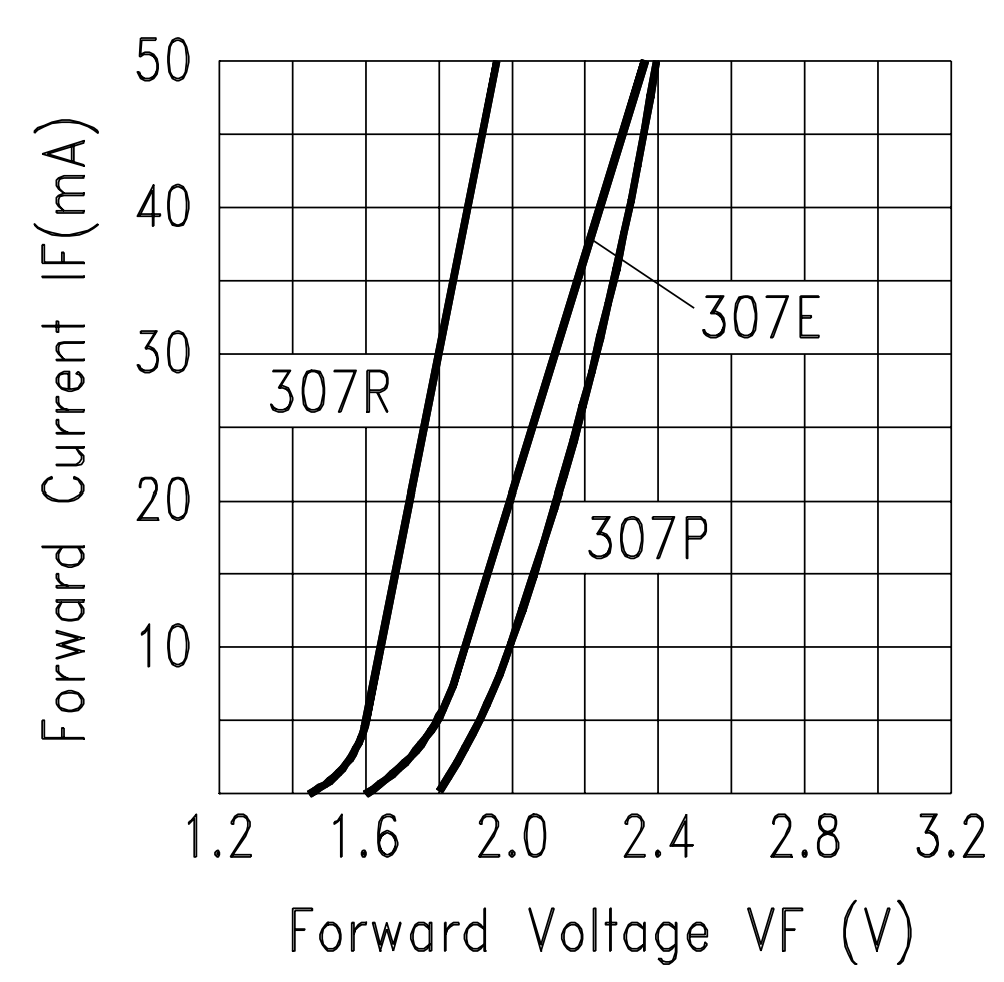
\includegraphics[width=4in]{iv_curve.png}
\end{center}

% =========================================================
\begin{partquestion}{basicloadline}
{Consider placing this LED in series with a fresh CR-2032 battery and a \qty{1}{\kilo\ohm} resistor. Use load-line analysis to determine the voltage across the diode and the current through the diode.}

\begin{answer}
A new CR-2032 battery will provide $V_{\text{batt}} = \qty{3}{\volt}$ of potential. The load-line equation for the circuit with a battery and \qty{1}{\kilo\ohm} resistor is found from Ohm's law:

\[
I_D = \frac{V_{\text{batt}} - V_D}{R} = (3 - V_D)\text{ mA}
\]

(Note the units are in mA since the resistor was in k$\Omega$.) We can plot this line on the on the graph in red. The $y$-intercept (at $V_D = 0$) is 3 mA, and the $x$-intercept is \qty{3}{\volt} (when $I_D = 0$).

\begin{center}
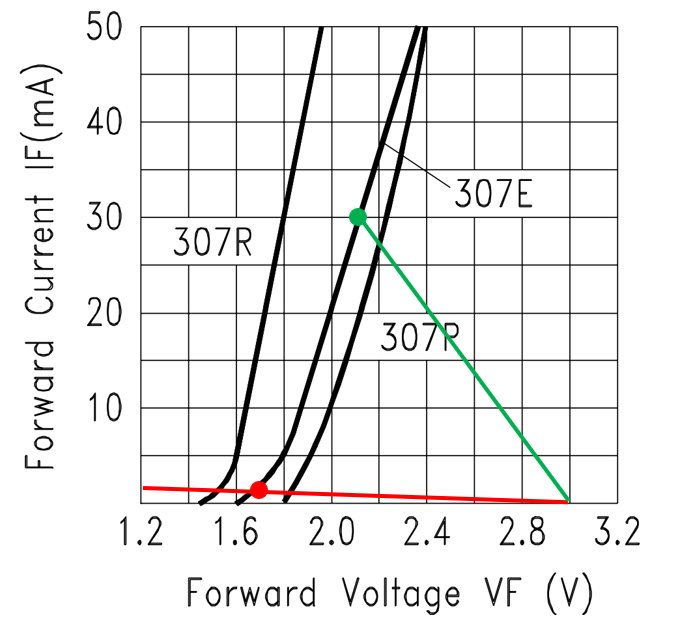
\includegraphics[width=4in]{iv_curve_traced.png}
\end{center}

This intersects the 307E curve at approximately:
\begin{itemize}
  \item Forward voltage: $V_D \approx \qty{1.7}{\volt}$
  \item Forward current: $I_D \approx \qty{1.3}{\milli\ampere}$
\end{itemize}
\end{answer}
\end{partquestion}

% =========================================================
\begin{partquestion}{ledbrightness}
{With the \qty{1}{\kilo\ohm} resistor, you may be disappointed by the LED brightness. Explain why that is.}

\begin{answer}
We are barely operating above the forward voltage cutoff level. The resulting low current (1.3 mA) is not a lot of current for typical LEDs such as this one, which are typically used in situations where there is an order of magnitude more current, providing a much brighter LED.
\end{answer}
\end{partquestion}

% =========================================================
\begin{partquestion}{resistorselection}
{After reviewing the salient details in the \href{https://www.jameco.com/Jameco/Products/ProdDS/697522.pdf}{data sheet}, again use load-line analysis to calculate a suitable resistor value that will continuously provide as bright an LED as possible while staying within the specified absolute maximum ratings. Make sure you choose a realizable resistor value (assume \href{https://asenergi.com/pdf/resistors/standard-resistor-values-e24.pdf}{E24 series}---also in Hambley Table B.1).}

\begin{answer}
According to the data sheet, the 307E LED is a Red Diffused LED with a High Efficiency Red source. The maximum rating at 25~°C for continuous forward current is given as 30 mA. From the I-V curve of the LED, this requires a LED forward voltage of about \qty{2.1}{\volt}. Using load-line analysis, we can draw a line between this point and the $x$-intercept (which remains at \qty{3}{\volt} since the battery is unchanged) in green. The slope is:

\[
\frac{\qty{0}{\milli\ampere} - \qty{30}{\milli\ampere}}{\qty{3}{\volt} - \qty{2.1}{\volt}} = -\qty{33.3}{\milli\siemens}
\]

The slope equals the negative reciprocal of the resistance:

\[
R = \frac{1}{\qty{33.3}{\milli\siemens}} = \qty{30}{\ohm}
\]

This represents a lower bound on $R$---any lower value would create a current higher than the maximum allowed forward current of 30 mA. Fortunately, the E24 series contains a \qty{30}{\ohm} resistor, so we can use that!
\end{answer}
\end{partquestion}

\end{mainquestion}
